\chapter{Contributions}
\section{Submodules and Specifications}
%%talk about the specs


The main focus of this thesis will be on two important submodules in charge of their load instructions:\\

\textit{Load Buffer} and \textit{Load Management Unit}.

\subsection{Load Management Unit}
%general


This module is in charge of handling the load operations.
Those can be strided or indexed.\\

Since the VPU is able to work out-of-order an ID system is necessary, so each instructions comes with an ID.
In particular the load operation come with the signal \textbf{seq\+id\+i}.
This signal contains all the informations about the issued load.\\

The main elements of this submodules are:
\begin{itemize}
    \item \textit{Shifter}: it is useful to have the first bit not in the MSB or LSB position.
    
    \item \textit{Compactor}: it is useful to compact all the valid elements. When the stride = 1 there is no use of the compactor.
    
    \item \textit{Aligner}: it is in charge to align the elements for the output (lane, bank and sub-bank).
\end{itemize}

\bigskip

%params
The main parameters defining this submodule are:
\begin{itemize}
    \item \textbf{MEM\+DATA\+WIDTH}: width of the chunk of data received from Avispado. The standard value is \textit{512}.
    
    \item \textbf{SEQ\+ID\+WIDTH}: width of the \textit{seq\+id\+i} that identifies the data coming from Avispado. The standard value is \textit{33}.
    
    \item \textbf{MAX\+NUMBER\+ELEMENTS}: maximum number of elements that can be encoded in the chunk of data received (64 when SEW = 8 bit). The standard value is \textit{64}.
    
    \item \textbf{MAVISPADO\+LOAD\+MASK\+WIDTH}: Indicates the maximum number of mask bits that are received with the data. Every bit of the mask represent a byte into the data. The standard value is \textit{64}.
    
    \item \textbf{NUM\+LANES}: number of lanes. The standard value is \textit{8}.
\end{itemize}

\subsubsection{Interface}
%interface
%%%%%%%%%%%%%%%%TABLE%%%%%%%%%%%%%%%%%%%%%%%

\begin{table}[H]
\centering
\begin{tabular}{|l|l|}
\hline
\rowcolor[HTML]{EFEFEF} 
\multicolumn{1}{|c|}{\cellcolor[HTML]{EFEFEF}Signal} & \multicolumn{1}{c|}{\cellcolor[HTML]{EFEFEF}Description}                      \\ \hline
load\+granted\+i    & a load is granted,\\
                    & it will have a certain sew\+i and stride\+i\\ \hline
load\+granted\+sb\+id\+i    & the id for the issued Load,\\
                            & can be issued up to 2 loads\\ \hline
indexed\+load\+granted\+i   & the granted load is indexed \\ \hline
load\+data\+valid\+i        & indicates if the data in load\+data\+i bus is valid\\ \hline
load\+data\+i               & data received from Avispado\\ \hline
seq\+id\+i                  & the sequence id (described below)\\ \hline
mask\+valid\+i              & validity of mask\+i signal\\ \hline
mask\+i                     & mask bits to mask load\+data\+i\\ \hline
sew\+i                      & identifies the size of each vector element\\ \hline
stride\+i                   & stride indicated in bytes\\ \hline
load\+data\+o               & output data sent to the lanes\\ \hline
load\+dvalid\+o             & indicates if the data in load\+data\+o bus is valid\\ \hline
mask\+o                     & mask bits to mask load\+data\+o\\
                            & it is needed also for not masked inst.\\ \hline
element\+ids\+o             & identifies each element sent in load\+data\+o\\ \hline
sb\+id\+o                   & identifies the instruction\\ \hline
vstart\+self\+o             & identifies the first valid element\\
                            & in the chunk of data received in load\+data\+i\\ \hline
vstart\+next\+o             & identifies the last valid element \\
                            & in the chunk of data received in load\+data\+i\\ \hline
min\+element\+id\+idx\+o    & index of the first valid \\
                            & element in elements\+ids\+o of each lane.\\ \hline
\end{tabular}
\end{table}


\subsubsection{Sequence ID}
The sequence id ID is very useful as the memory system does not guarantee the in-order arrival of elements. So this signal contains all the info needed to correctly elaborate the data.\\

It is composed as:
\begin{itemize}
    \item \textbf{seq\+id\+i[4:0]} = \textit{v\+reg}, identifies the logical vector register that the data should be written to;
    
    \item \textbf{seq\+id\+i[15:5]} = \textit{el\+id}, identifies the lowest valid element id contained in the chunk of data being transmitted;
    
    \item \textbf{seq\+id\+i[21:16]} = \textit{el\+off}, identifies the offset in the chunk of data being transmitted.
    
    \item \textbf{seq\+id\+i[28:22]} = \textit{el\+count}, identifies the number of valid elements being transmitted. Masked elements are valid elements; 
    
    \item \textbf{seq\+id\+i[32:29]} = \textit{sb\+id}, sb\+id of the load instruction that requested the data.
\end{itemize}


\subsubsection{Handshake}
The handshake protocol with the different components is as important as the data manipulation. Following, there is a simple example with stride equal to 1 and offset = 0 (so, no manipulation on the data in input), furthermore, we do not focus on how long is the vector (VLEN) so the number of elements passed from Avispado is arbitrary fixed.

\begin{enumerate}
    \item Up to 2 load are granted from the Memory Unit with the load\+granted\+i signal, and the information of sew and stride of the relative instruction are passed;
    
    \item Avispado sends the data and the seq\+id\+i with its seq\+id;
    
    \item The next clock cycle the data is on the output for the Vector Lane;
    
    \item When a load is finished, another load can be granted.
\end{enumerate}

\begin{figure}[H]
    \centering
    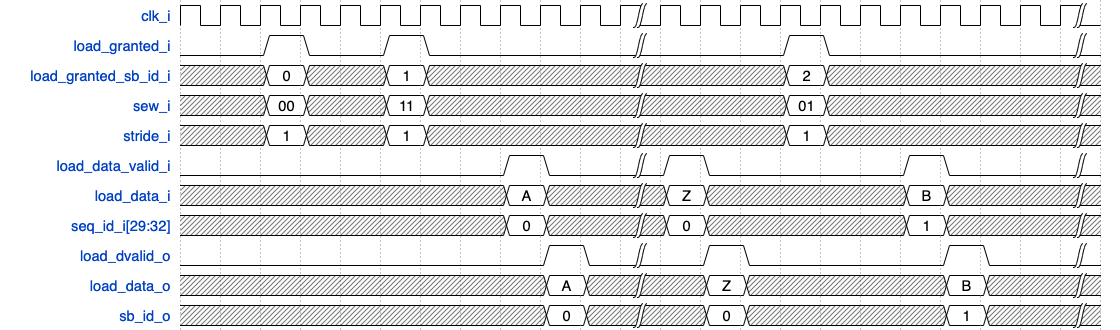
\includegraphics[scale = 0.35]{Chapter_2/img/lmu-time.png}
    \caption{Timing Diagram unit-strided load for the LMU}
    \label{lmu-time}
\end{figure}

In Figure \ref{lmu-time} it is possible to see an example for a unit-strided load. This is a simple load, and its behaviour will be discussed in the following section.

\subsubsection{Strided Load}
In this case all the valid elements are separated by a constant stride. If the stride is equal to 1, then is called unit-stride.\\

Figure \ref{lmu-strided} shows how the LMU works in this case.\\
The parameters (defined in the seq\+id\+i) are defining the elements to consider.
\begin{figure}[H]
    \centering
    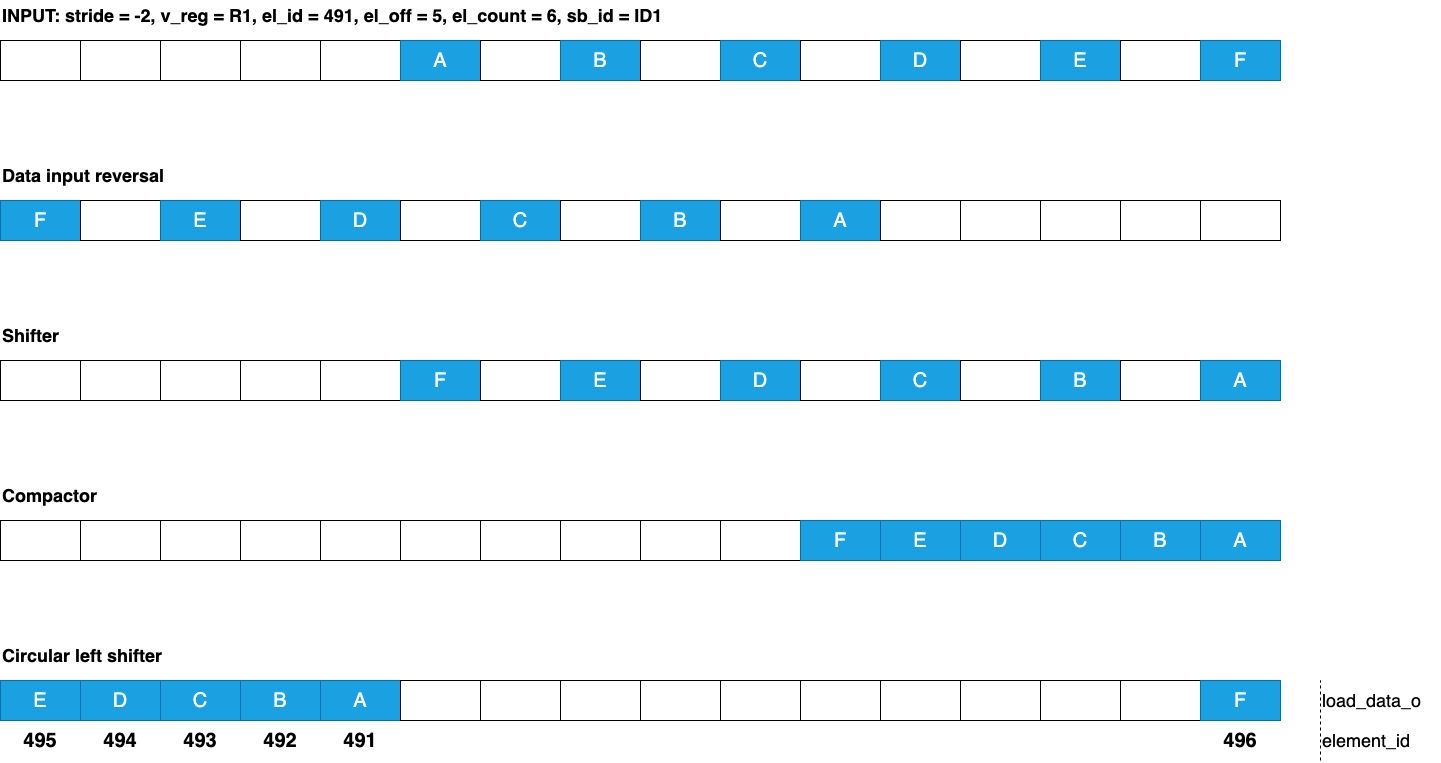
\includegraphics[scale = 0.25]{Chapter_2/img/lmu-strided.png}
    \caption{Strided load handled by the LMU}
    \label{lmu-strided}
\end{figure}

\subsubsection{Indexed Load}
It is also possible to load values in an indexed way. This means that only one element at time is sent, and so the number of valid elements needs to be = 1.\\

In Figure \ref{lmu-indexed} it is possible to see an example for a simple indexed load.

\begin{figure}[H]
    \centering
    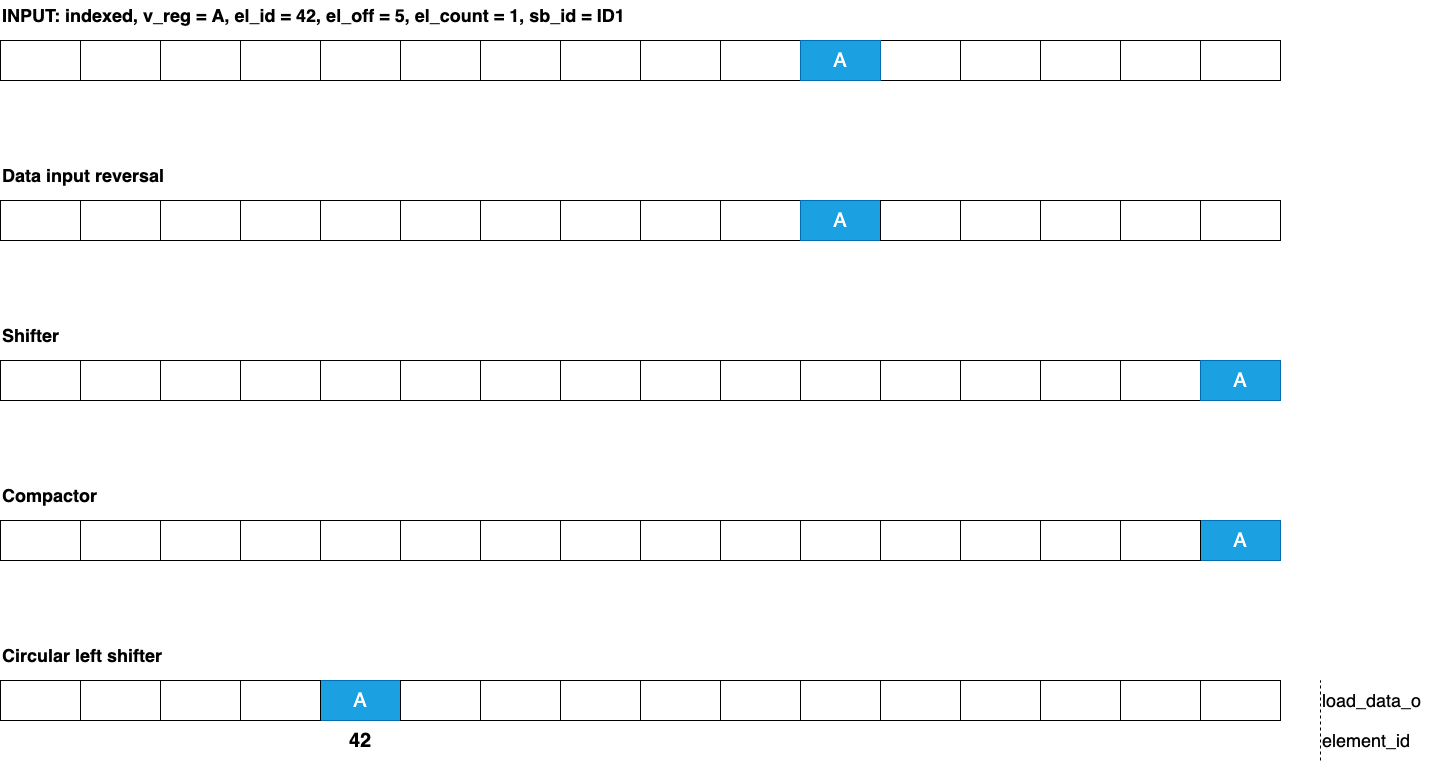
\includegraphics[scale = 0.25]{Chapter_2/img/lmu-indexed.png}
    \caption{Indexed load handled by the LMU}
    \label{lmu-indexed}
\end{figure}

\subsubsection{Masked Load}
All the load operations can be masked. This does not change the number of valid elements, but at the end of the process they will not be sent.\\


In Figure \ref{lmu-masked-stride} it is possible to see an example of the simple strided-load used before, but this time, with a mask.

\begin{figure}[H]
    \centering
    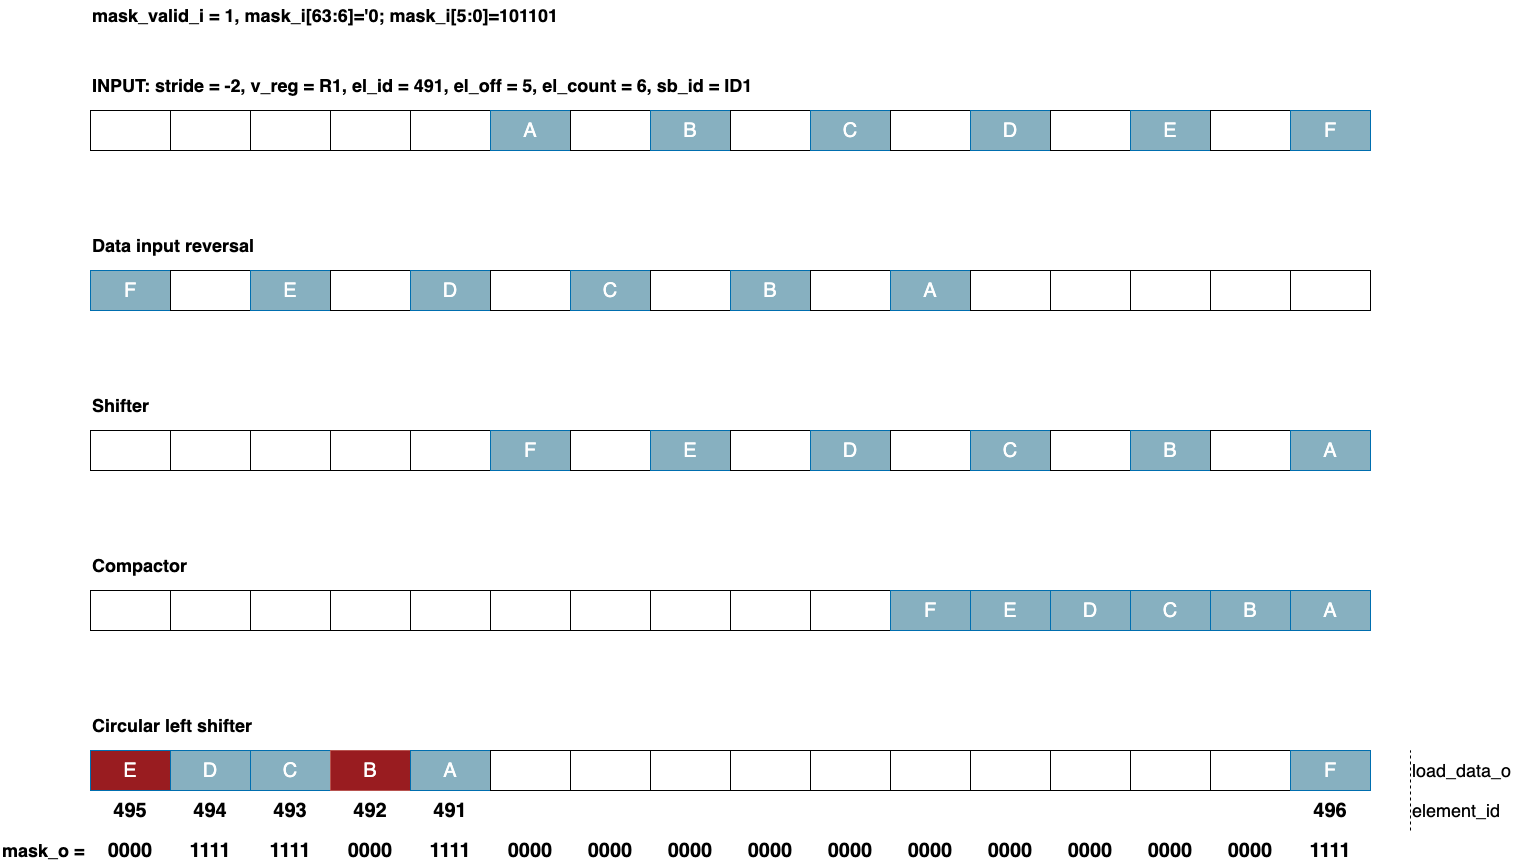
\includegraphics[scale = 0.25]{Chapter_2/img/lmu-masked-strided.png}
    \caption{Strided load, with mask, handled by the LMU}
    \label{lmu-masked-stride}
\end{figure}

\subsection{Load Buffer}
The second submodule that is mainly in charge of a load operation is the Load Buffer.\\
Its function is writing the data sent by Avispado to the Vector Register File. The data can come from different instructions inflight, and the Buffer will always try to optimize and group the data to write.\\

The LMU receives full cache lines of 512 bits from Avispado and forwards them to the corresponding Load Buffer for each lane (64 bits max per lane), depending on the seq\+id\+i. The position of the data into the LB will be determined by the element ID.\\

Up to 2 loads can arrive, but they can come out-of-order, although the implementation will be parameterized to accept N loads in flight.
\subsubsection{Interface}
The Load Buffer is connected with a lot of modules. From the \emph{Vector Lane} it receives the clock and the reset and communicates if there is a load inflight; with the \emph{LMU} it exchanges all the data; from \emph{Avispado} it knows if te operation has terminated; the request handshake is handled with the \emph{Memory Queue}; the data goes to the \emph{Vector Register File}, synchronizing via the internal \emph{Finite State Machine}; finally it can commit the result with the \emph{Commit Unit}.\\

A simple structure is represented in Figure \ref{lb-if}.

\begin{figure}[H]
    \centering
    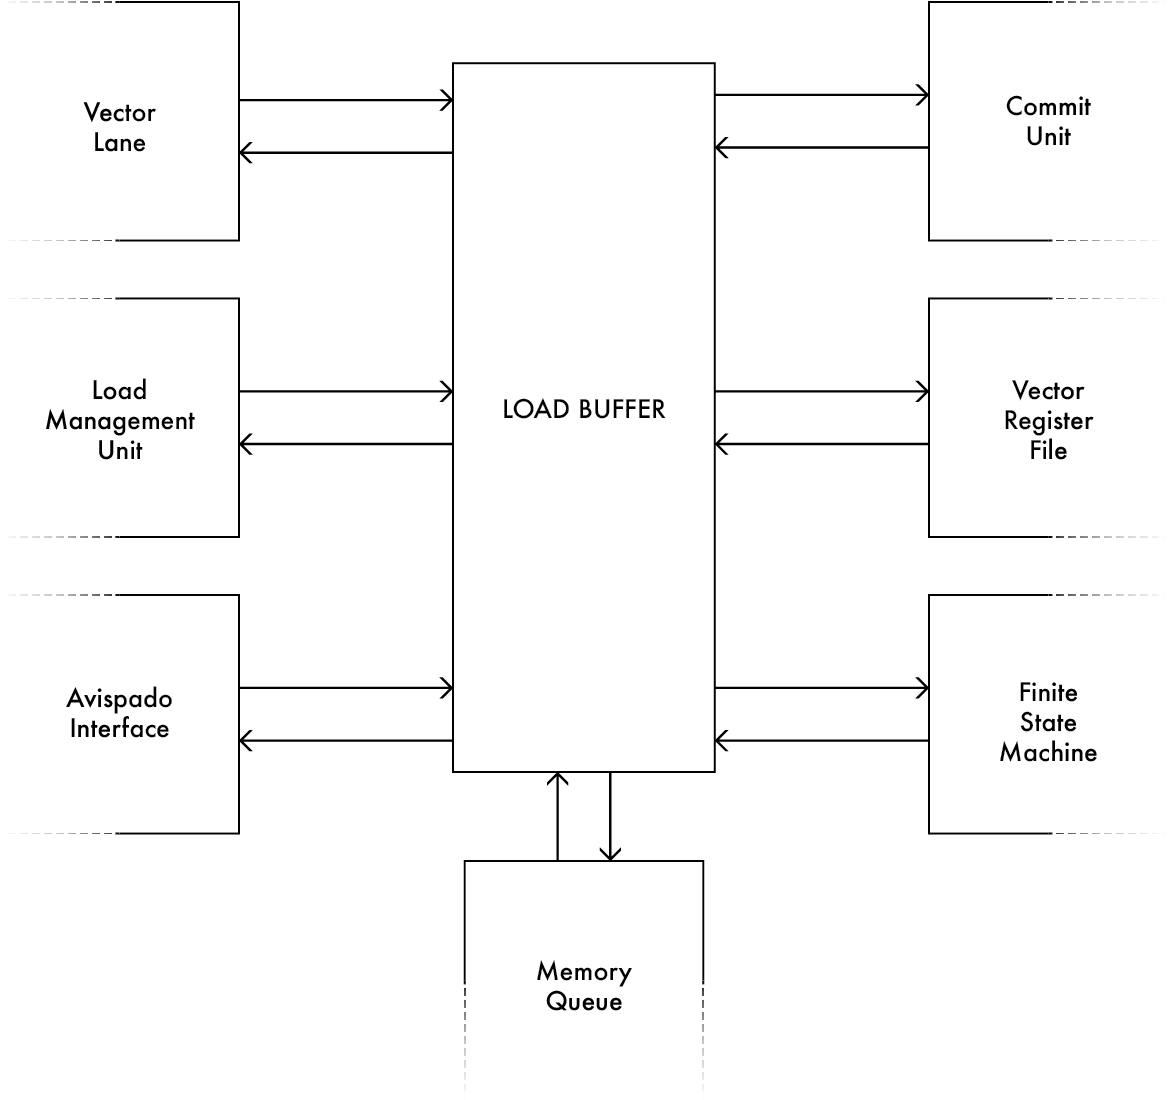
\includegraphics[scale = 0.4]{Chapter_2/img/lb-if.png}
    \caption{Load Buffer's interfaces}
    \label{lb-if}
\end{figure}

\subsubsection{Structure}
There is a Load Buffer of each lane and there are 3 layers to buffer the elements. The layers are divided by the concept of Element Group. In fact the elements cannot be disposed in every combination, but every element, based on its element ID, has an exact location (based also on the sew).\\

In Figure \ref{gen-ex} it is possible to see a general connection between the LMU and the various Load Buffers.\\

\begin{figure}[H]
    \centering
    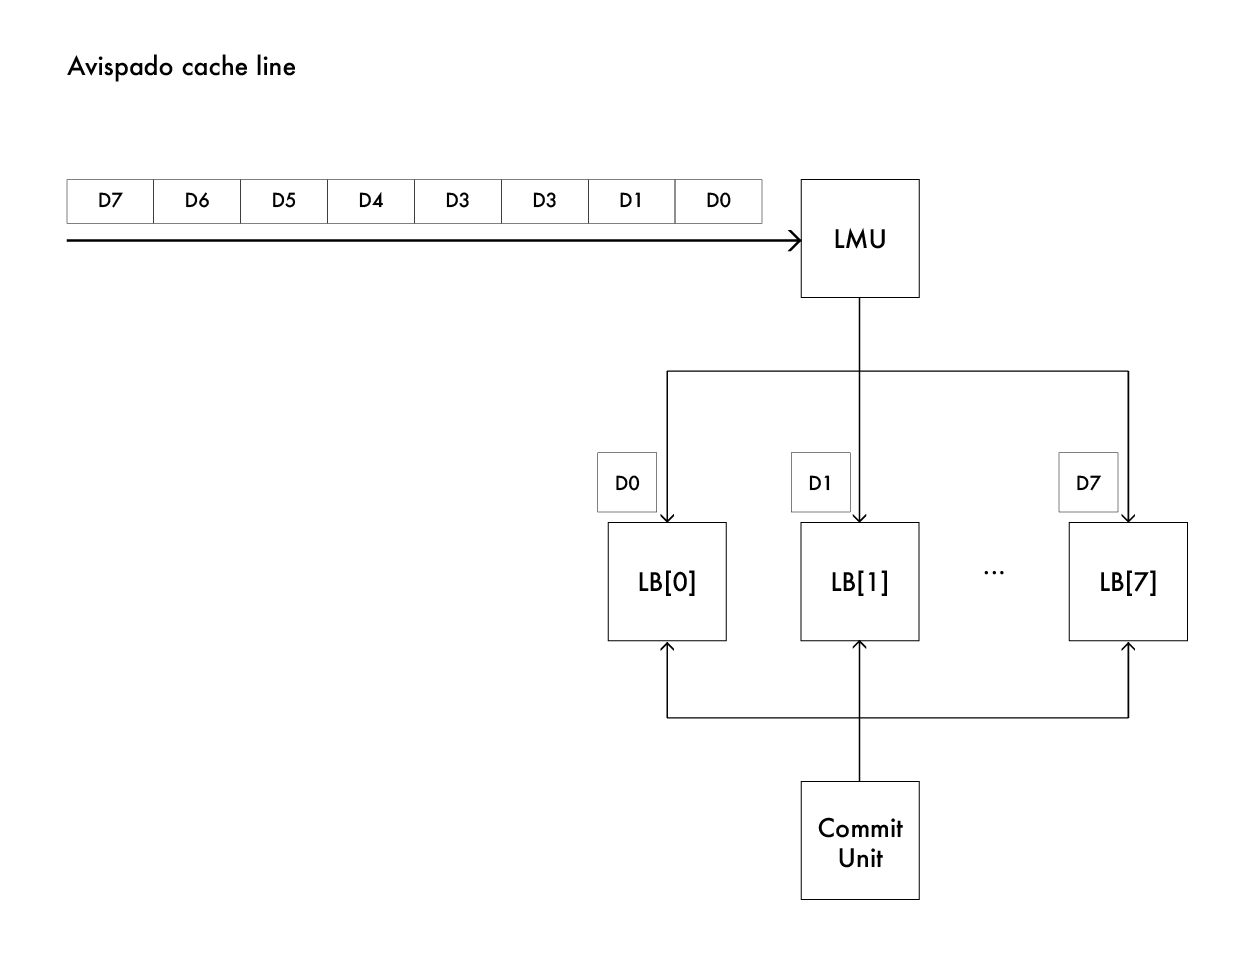
\includegraphics[scale = 0.5]{Chapter_2/img/cache-to-lb-gen-ex.png}
    \caption{Data through the LB}
    \label{gen-ex}
\end{figure}


In Figure \ref{lb-genz} there is an example for the disposition of the elements of 64 bit. It is also important to say the number of bit for each element group stays the same, this means that the number of element depends on the sew.\\


\begin{figure}[H]
    \centering
    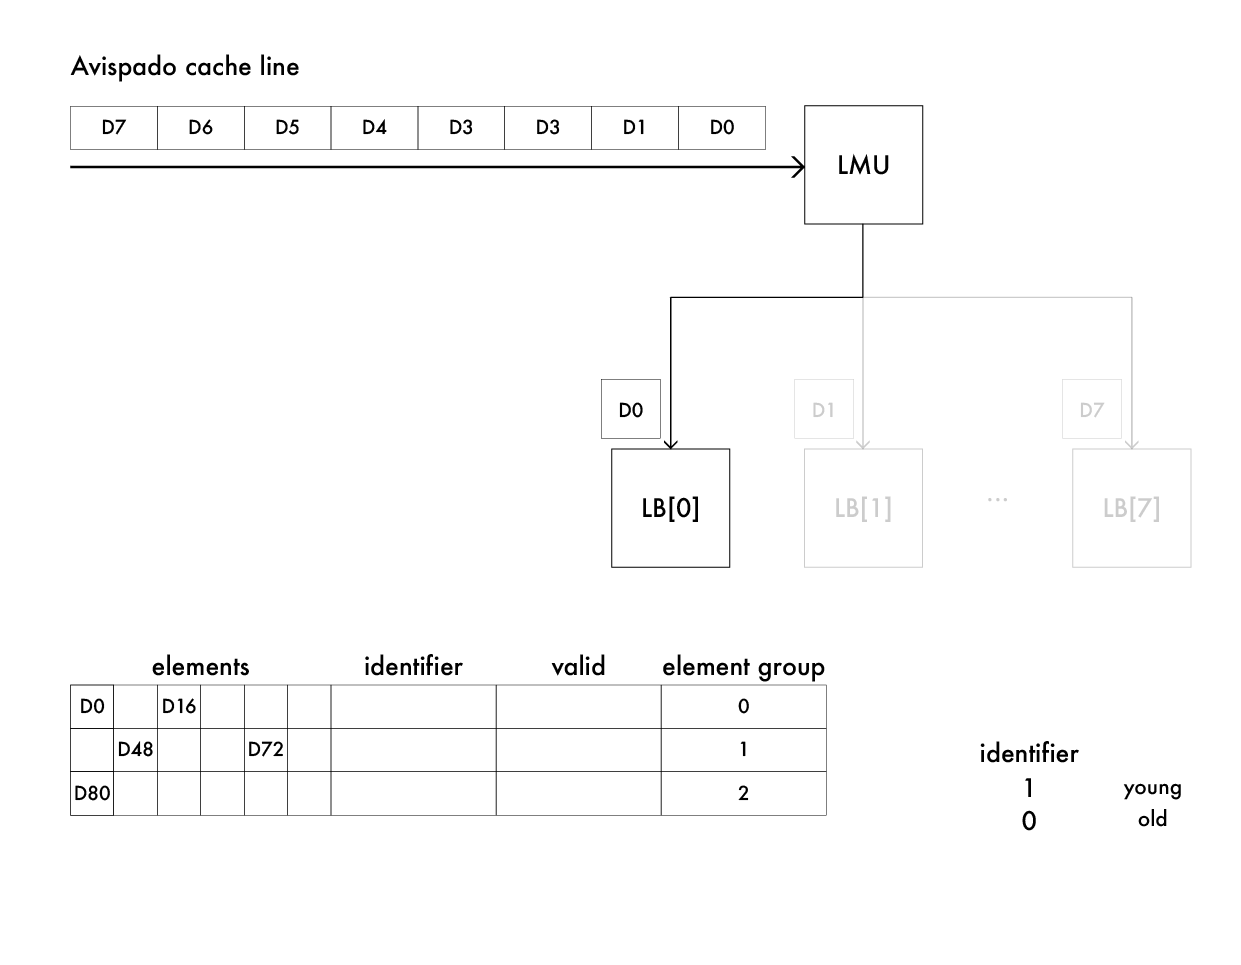
\includegraphics[scale = 0.4]{Chapter_2/img/cache-to-lb-genz-ex.png}
    \caption{General case for the LB}
    \label{lb-genz}
\end{figure}

The layers of the LB are mainly composed of 4 parts:
\begin{itemize}
    \item Elements: the elements in the buffer, they are always 512 bit, so 5 elements with sew = 64, 10 elements with sew =32 and so on;
    
    \item Identifier: identifies the elements coming from the young or the old load;
    
    \item Valid: identifies if the elements are valid;
    
    \item Element Group: identifies the eg, it is assigned by considering the VRF structure.
\end{itemize}

\subsubsection{Retry}
There are cases in which 3 layers are not enough to store all the elements. Indeed it is possible that more elements have the same position and so also 4 element can cause a problem, if they try to fit.\\

This case is handled with a retry mechanism:\\
an element is discarded and a new request is made to Avispado, to  notify the retry.\\

Is important to understand the element to discard when there is a retry, wheather it is a new or an old one.\\

There are 4 possible cases:
\begin{enumerate}
    \item if the incoming data comes from the young load and the buffer does only contain data from the same load, it will be discarded the data with the highest element group;
    
    \item if the incoming data comes from the young load and the buffer contains data from both the oldest and youngest loads, it will discard the incoming data;
    
    \item if the incoming data comes from the old load and the buffer only contains data from the same load, it will be discarded the data with the highest element group;
    
    \item if the incoming data comes from the old load and the buffer contain data from both the oldest and youngest loads, it will discard the data inside the buffer, the one from the young load.
\end{enumerate}



\subsubsection{Flow}
In Figure \ref{lb-flow} it is possible to see a simple scheme of the LB's behaviour.

\newpage
\begin{figure}[H]
    \centering
    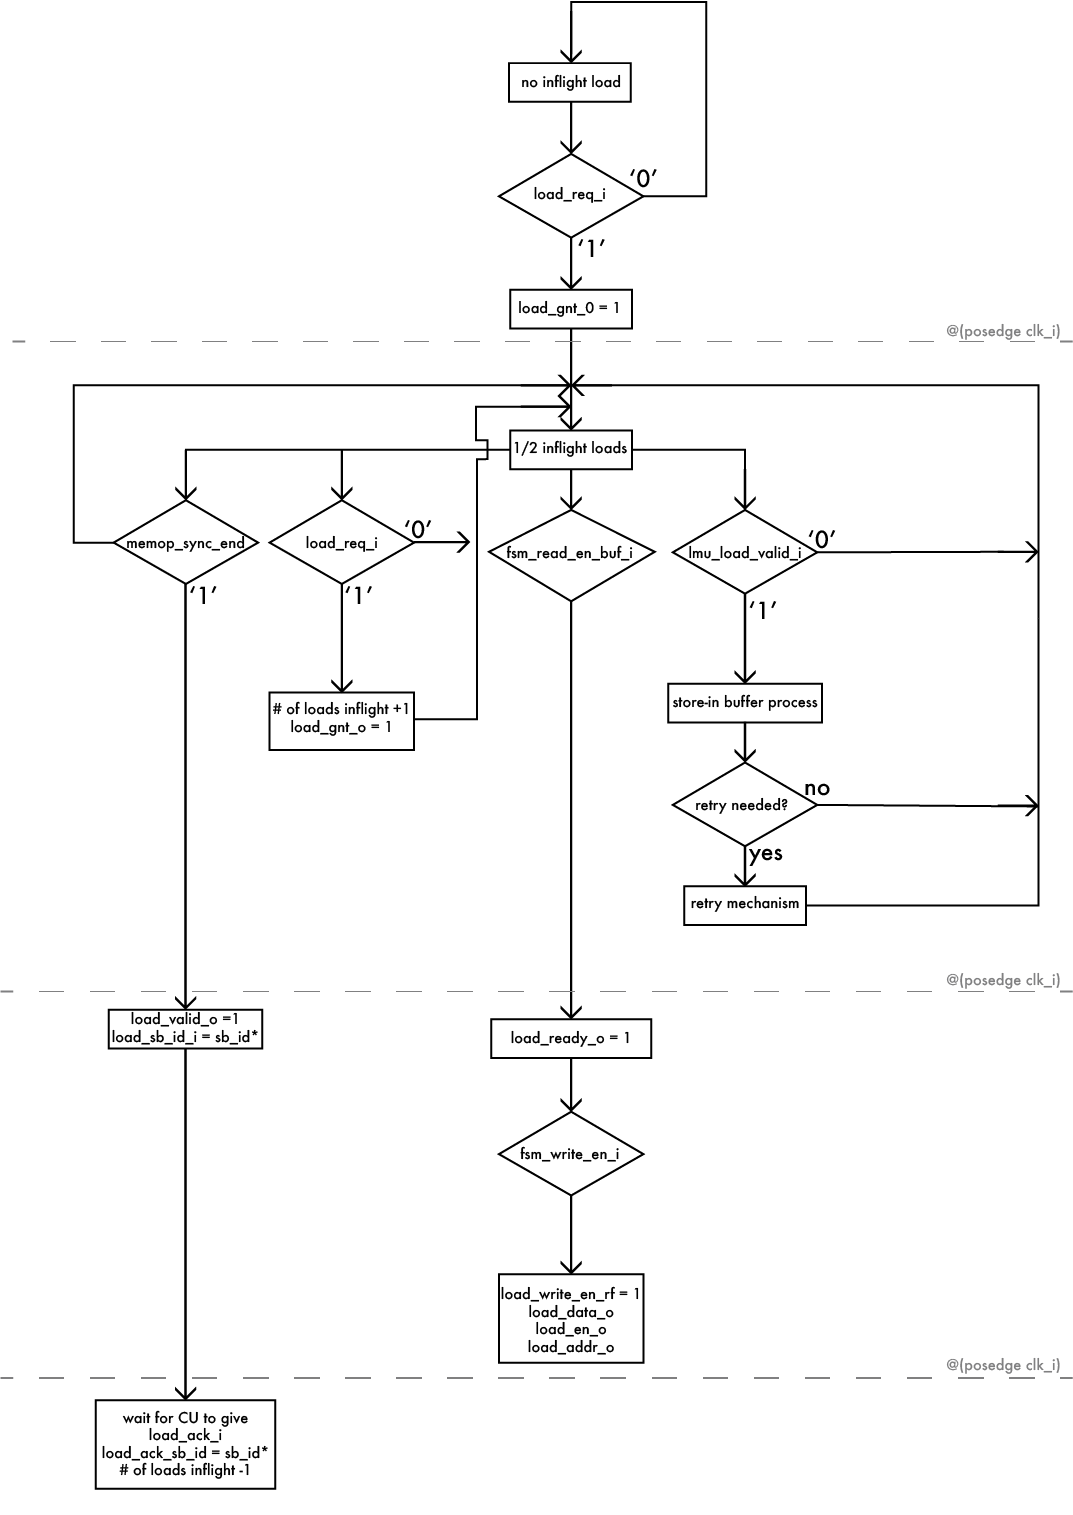
\includegraphics[scale = 0.8]{Chapter_2/img/lb-flow.png}
    \caption{Working flow of the Load Buffer}
    \label{lb-flow}
\end{figure}

Following the scheme it is possible to understand the main working flow of the Load Buffer.\\
When it receives a request it grantees it, then it can have different possibilities.\\
It can receive the data, and in case activate the retry mechanism, or it can receive another request (up to 2 inflight loads at once) or it can receive a \emph{memop\+sync\+end} and then continue the process to finish the load.\\
Or it is possible \emph{fsm\+read\+en\+buf\+i} arrives and the LB can write the data in output.\\


\section{Verification Plan}
In order to have a better approach with the verification of a design, it is important to define a Verification Plan.\\
There are many ways to accomplish it, and most of the times they can be automatized to better perform in long term support of them. In this specific case, the Verification Team was working along with the Design Team to produce better specifications and not only to test a completed design. This means that the Verification Plan is done following the general rules to have a good value in future, but it is not entirely defined a priori.\\

It was previously defined to create the UVM structure and led to the development of all the tools for the verification. \\
Defining the approach to have does also mean to defining the tools that will be used, in fact, many different of them were created:
\begin{itemize}
    \item \textbf{UVM}: is the structure described earlier, used to stimulate and test the DUT;
    
    \item \textbf{checkers}: are mainly composed by assertions, some really powerful statements used to define the constraints of the DUT's behaviour. \\
    They can be used in different approaches. Later on this chapter it will be discussed their use as Functional or Formal tools;
    
    \item \textbf{coverage}: is the driver of the plan. It says were to work, and were there are tests to perform. 
    
\end{itemize}
\subsection{Test Plan}
In order to have a good coverage of the cases, and good reports to find bugs, it is very important to have a test plan.\\

The test plan defines all the different cases to test for a submodule or for the entire VPU. This means trying to find all the different corner cases stimulating the DUT.\\

If there is the possibility a good test plan only includes different sets of stimulus, in this way an easy implementation is possible. But this situation does not cover all the possible cases. For instance, not every case could be tested in a submodule of the VPU only modifying the inputs from the scalar core.\\
Which means that sometimes it is necessary to create some modified settings, to create the correct environment for the test.\\

It was created a test plan to stress the load operations. Those are affecting a lot of part of the VPU, but the focus will be on the Load Buffer, mainly.\\

\subsubsection{test on consecutive elements}
The first test planned was a simple test about consecutive elements, this means all the elements are sent in order. Of course this is a simple case, and it is thought to test if all the chain to the effective load are working. In fact it is a control test.\\

The only constraint meant to be in this test is the sequentiality of the elements.\\
An example could be the one represented in Figure \ref{cache-to-lb-seq-ex}.


\begin{figure}[H]
    \centering
    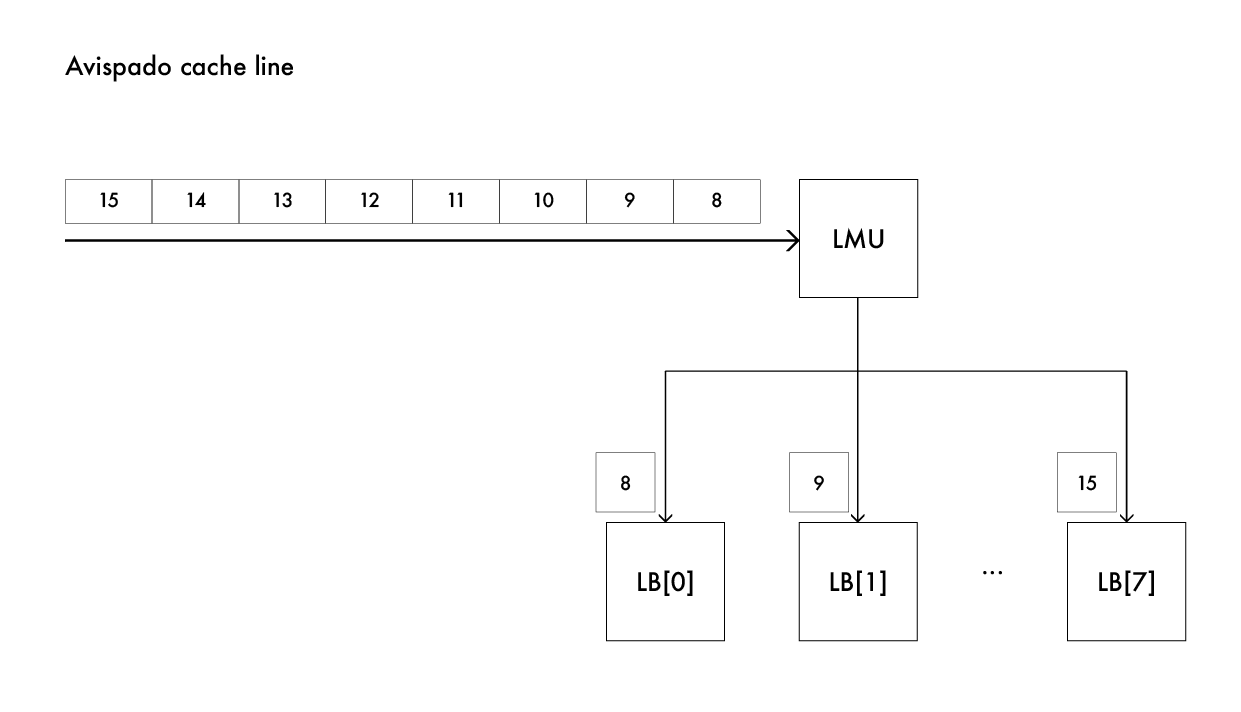
\includegraphics[scale = 0.6]{Chapter_2/img/cache-to-lb-seq-ex.png}
    \caption{Sequential inputs from avispado}
    \label{cache-to-lb-seq-ex}
\end{figure}

\subsubsection{test on random values}
The second kind of test to implement is for sure the random test. This will stress the ability to use different elements ID and different loads at the same time. In this way all the handling for the positions, calculated based on the load and on the element ID, is stressed.\\

It was created a special modality to constrain the randomness to the possible values. This was implemented in the UVM using the configurations for the sequence.\\

An example on random inputs from the same load could be the one represented in Figure \ref{cache-to-lb-rnd-ex}.

\begin{figure}[H]
    \centering
    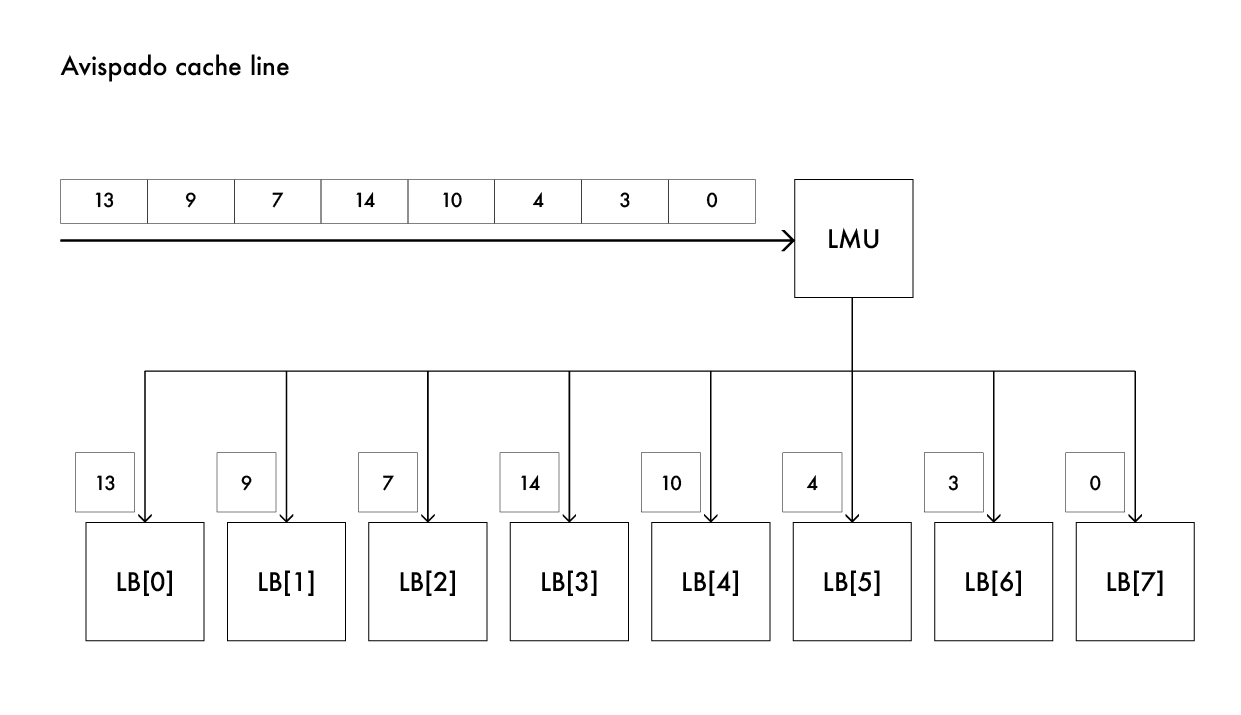
\includegraphics[scale = 0.6]{Chapter_2/img/cache-to-lb-rnd-ex.png}
    \caption{Random inputs from avispado}
    \label{cache-to-lb-rnd-ex}
\end{figure}

It is also possible to have inputs from two loads, as in Figure \ref{cache-to-lb-ooo-ex}.

\begin{figure}[H]
    \centering
    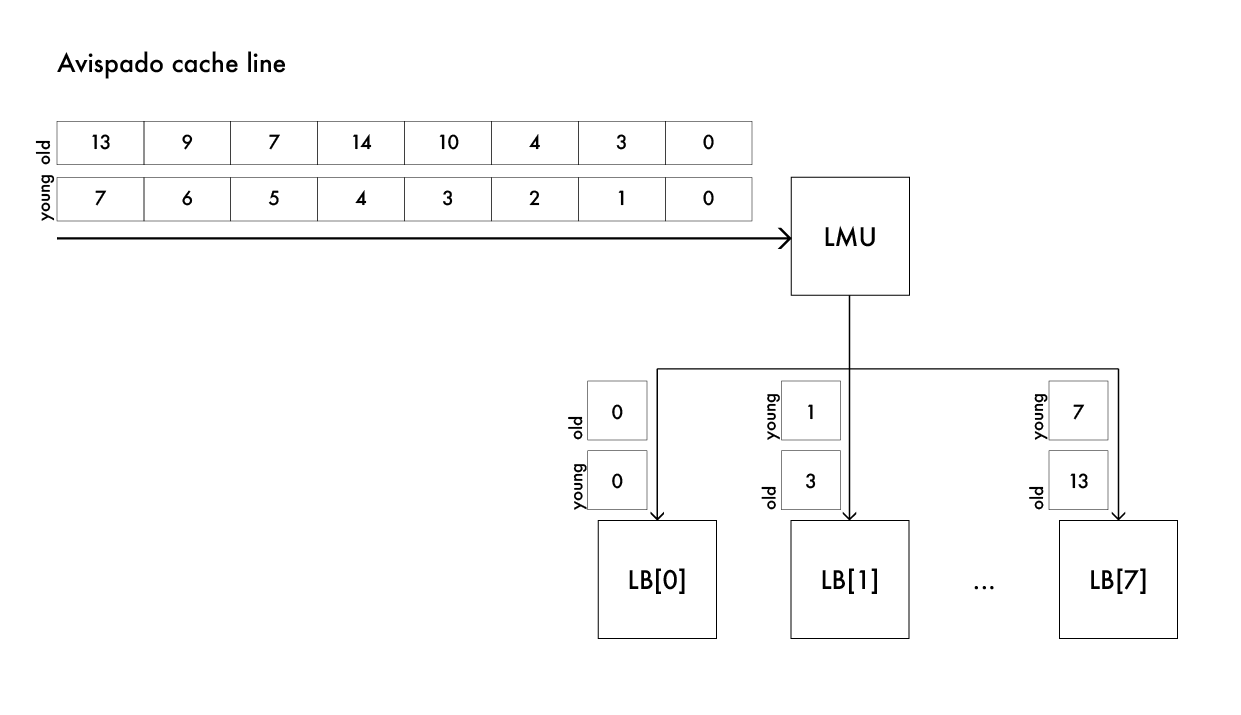
\includegraphics[scale = 0.6]{Chapter_2/img/cache-to-lb-ooo-ex.png}
    \caption{Random inputs from two loads}
    \label{cache-to-lb-ooo-ex}
\end{figure}

\subsubsection{test on splitted elements} 
A very interesting case is revealed when studying the positions.\\
Let's take into account a line of elements sent by the LMU to the Load Buffer. In this case the sew needs to be different from 64, so the case will use sew = 32.\\

The data sent will be sequential starting from 65 to 80. In this way it is possible to test if the output is disposed correctly and so if the Load Buffer for the Lane[0] store 80-65 as values.\\

An example could be the one represented in Figure \ref{cache-to-lb-split-ex}. It also shows how the input is splitted in the LB.

\begin{figure}[H]
    \centering
    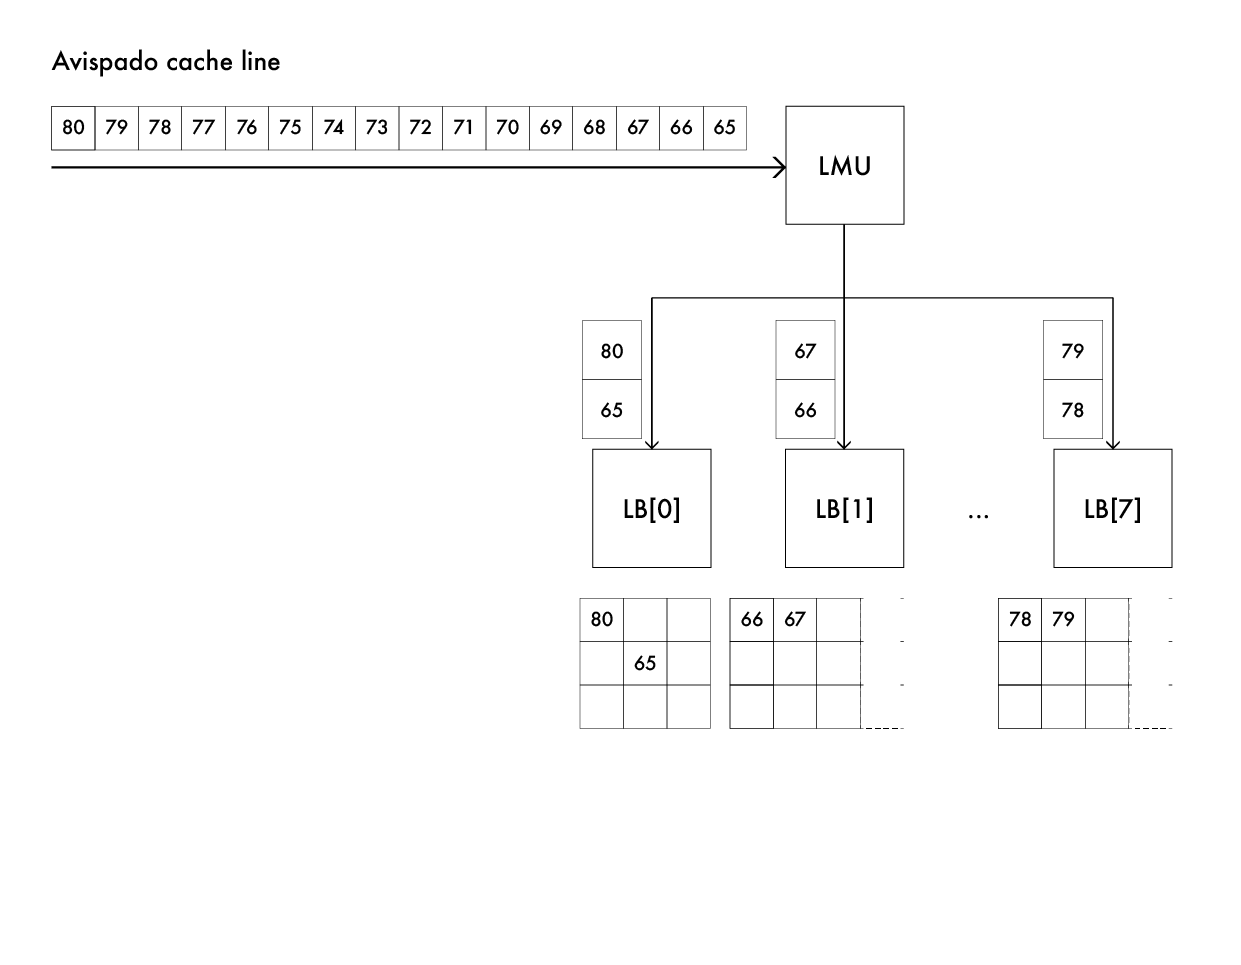
\includegraphics[scale = 0.6]{Chapter_2/img/cache-to-lb-split-ex.png}
    \caption{Input splitted into the LB}
    \label{cache-to-lb-split-ex}
\end{figure}

\subsubsection{test on retries}
The last test typology is about the retry mechanism. This occurs when all the tree lines are fulled with an element in the same position, and thena fourth elements arrives, this means the Load Buffer doesn't have another position for the element, thus one of the elements needs to go back to the sender and a new request is made.\\

Considering sew = 64, there are different versions about this test: it can be a simple in order retry with elements 0-40-80-120-... as inputs, it can be out of order as 0-40-120-80-..., or it can be with two different loads.\\

The easy example is represented in Figure \ref{cache-to-lb-ret-ex}. 0-40-80 are already filling the spots where 120 will try to fit. So a retry is needed, discarding 120.

\begin{figure}[H]
    \centering
    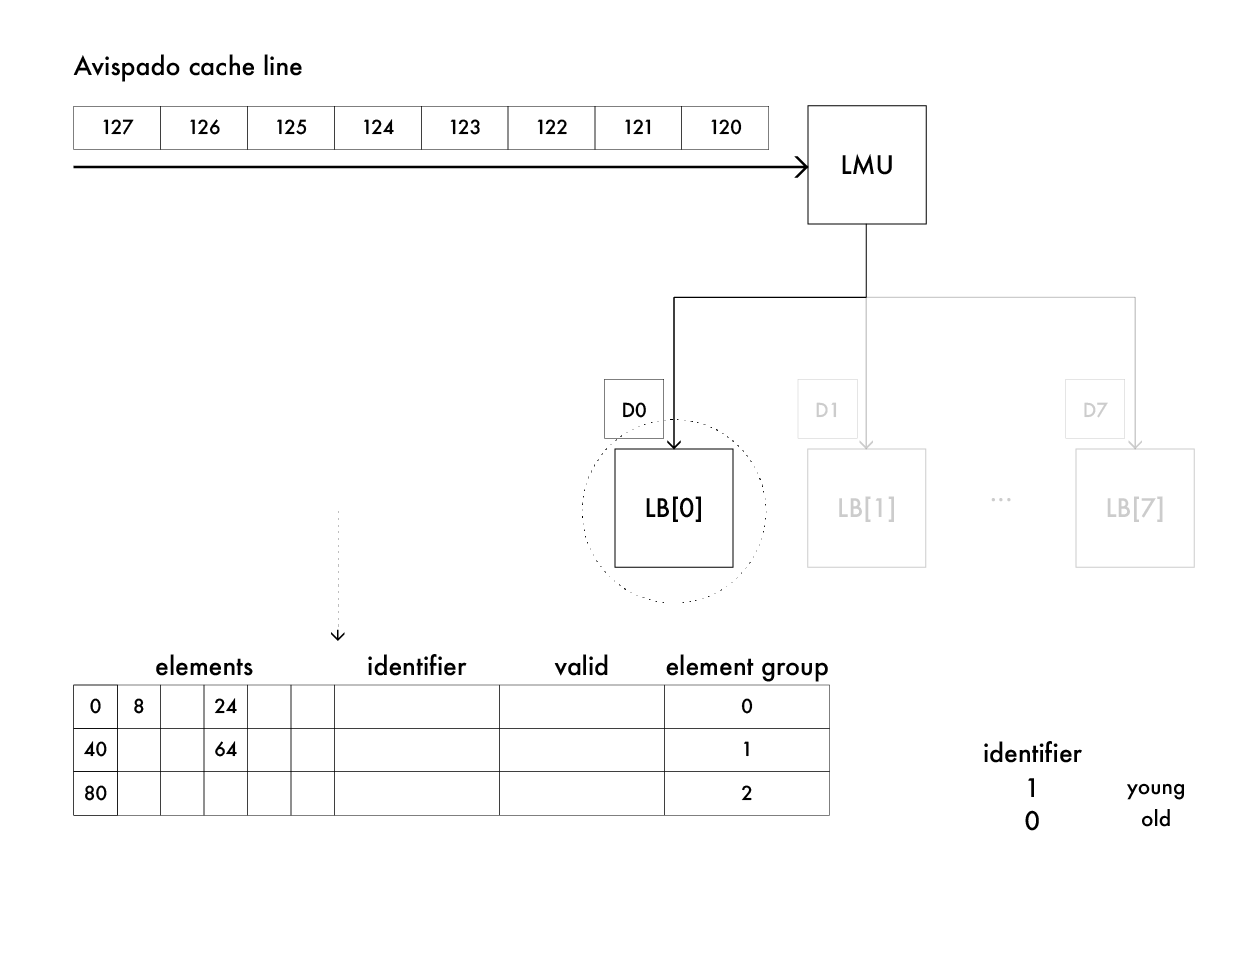
\includegraphics[scale = 0.5]{Chapter_2/img/cache-to-lb-ret-ex.png}
    \caption{Stimulated retry}
    \label{cache-to-lb-ret-ex}
\end{figure}


The out-of-order example is represented in Figure \ref{cache-to-lb-ooo-ret-ex}. 0-40-120 are already filling the spots where 80 will try to fit. So a retry is needed, discarding 120, and taking 80.

\begin{figure}[H]
    \centering
    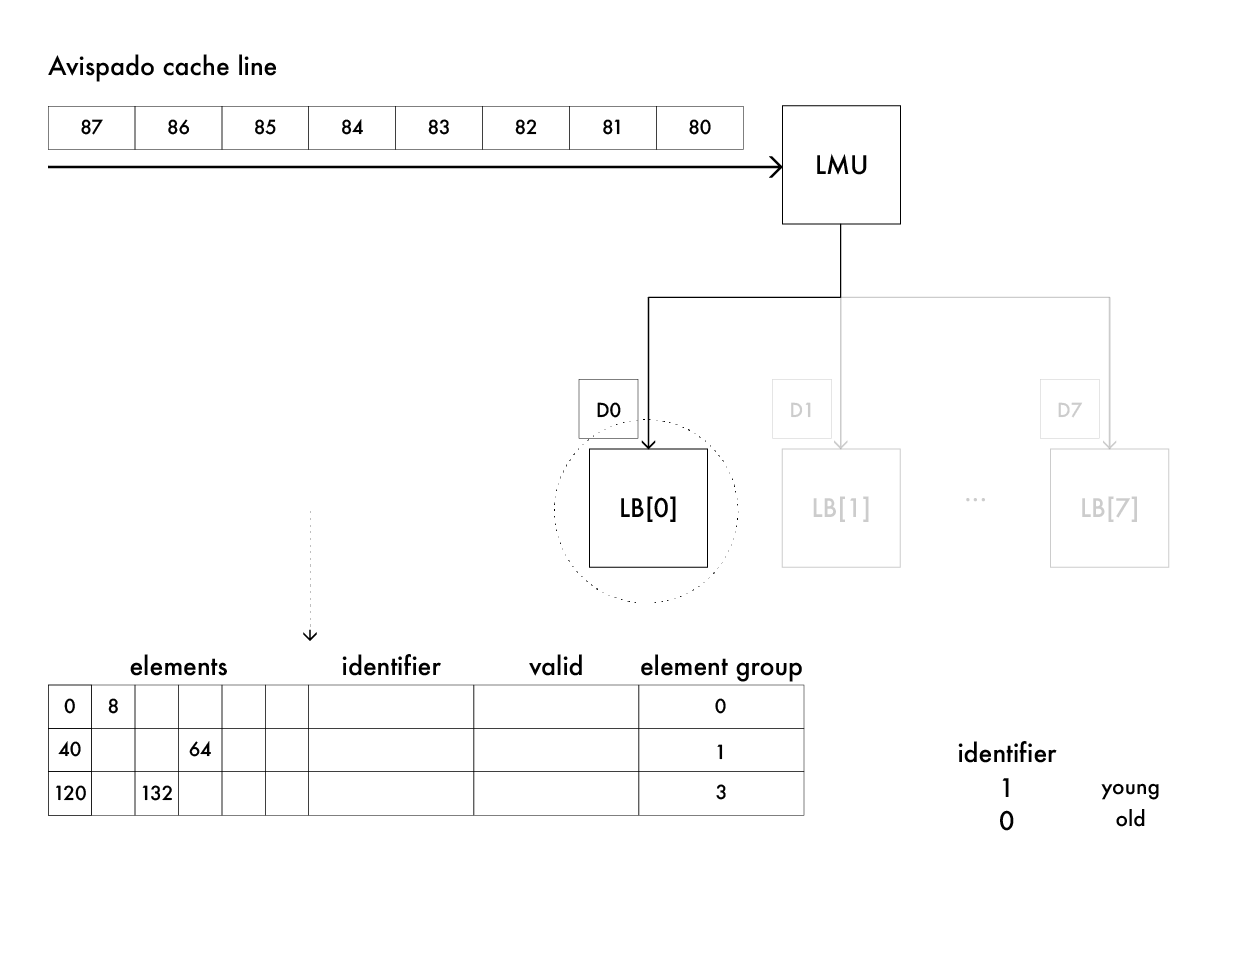
\includegraphics[scale = 0.5]{Chapter_2/img/cache-to-lb-ooo-ret-ex.png}
    \caption{Stimulated retry with out-of-order values}
    \label{cache-to-lb-ooo-ret-ex}
\end{figure}



\section{Functional Verification}
The test executed are just the base for a verification. It can be defined Functional Verification the process to verify a design agaist its specifications.\\

The approach is normally to define some functionalities and then compare them to the design. This of course is the crucial part, because it is not always obvious how a specific case works. Also there are different ways to test those functionalities.\\

\subsection{Scoreboard}
As saw into the test plan, an easy way to test the results is the scoreboard, thus to have a predicted value and then to compare it against the calculated one.\\

Before the work of this thesis a scoreboard for the entire UVM was already implemented. Let's now analyze a little bit how it works and why it was useful to develop other tests.

\subsubsection{Spike}
Spike is a RISC-V ISA Simulator and it implements a functional model of one or more RISC-V harts. For this specific project it was extended to support the vector extension.\\
It is used first to simulate the Avispado core, then the result is feed to the VPU and to the Spike vector extension. Finally the results are compared. A simple scheme is represented in Figure \ref{bin-to-log}. \\

\begin{figure}[H]
    \centering
    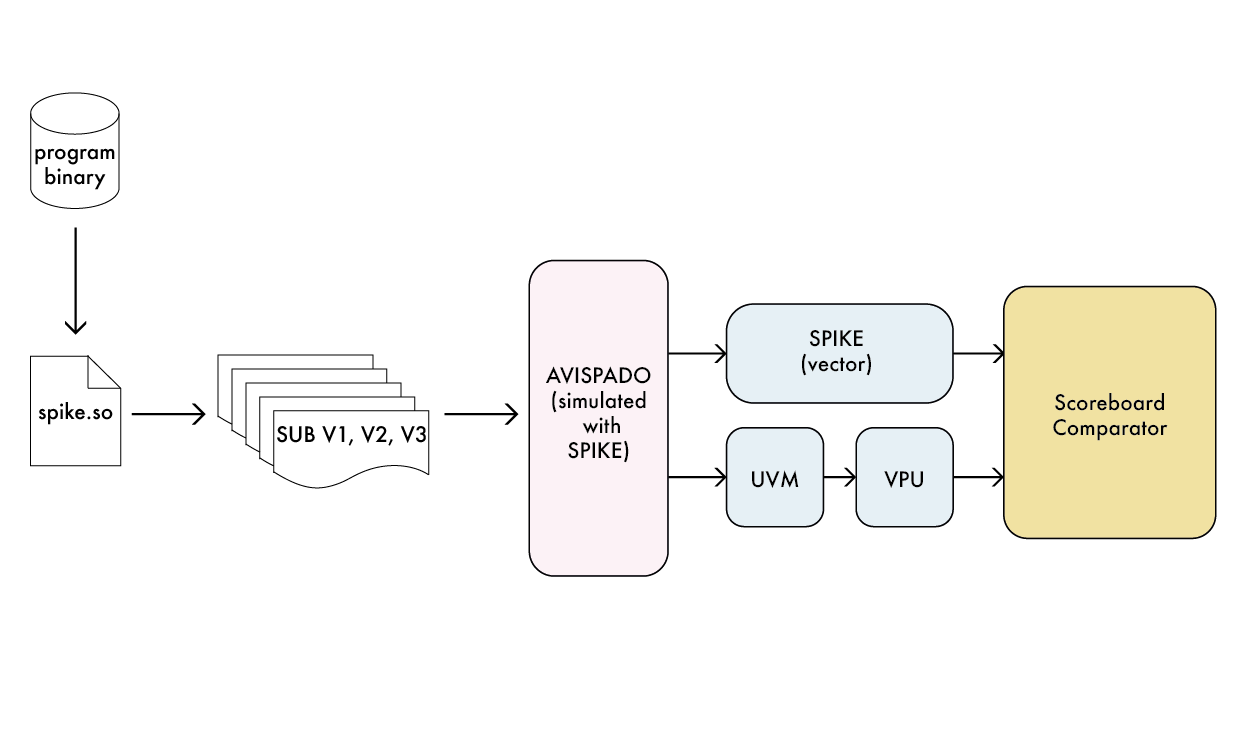
\includegraphics[scale = 0.5]{Chapter_2/img/bin-to-log.png}
    \caption{Simulation path}
    \label{bin-to-log}
\end{figure}

This kind of tool is very useful when running tests because it is faster than a specific test for each component the test is stressing, and at the same time can give hints about the working condition. Of course it is just a first step, because it will be hard to find a bug using only the comparison with the final result.\\

\subsubsection{Load Management Unit's scoreboard}
The aim of this thesis was principally based on testing the Load operations, so a scoreboard for the LMU was created.\\

Recalling the LMU working model, it first takes into account the stride, reversing the data in case of negative stride, then the data is positioned correctly again, then it is compacted considering the stride, and finally it is aligned to match with correct ID.\\

In high level it was done using vectors, and a couple of steps were merged together. It is possible to see below the pseudo code represntig the implementation in this way.

\begin{lstlisting}[language=Verilog,style=verilog-style, backgroundcolor=\color{lyel_palette}, frame=tlb]
        x=new[N_ELEMENTS][SEW];
        y=new[N_ELEMENTS][SEW];

        //first assignement
        x[N_ELEMETS][SEW] = load_data_i[N_ELEEMTS*SEW]

        //consider the stride
        if(stride<0 && !is_indexed)
            y[i] = x[-i];
        else
            y[i] = x[i];
        

        //from # of bytes to # of elements
        local_stride = mod(local_stride * 8 / SEW);

        //concatenate the data according to stride 
        x[N_ELEMENTS-1-i] = y[(N_ELEMENTS-1-i*local_stride-OFFSET)%N_ELEMENTS];

        //shift the data according to EL_ID
        k = EL_ID % N_ELEMENTS;
        
        y[(N_ELEMENTS-1-(k+i))%N_ELEMENTS] = x[(N_ELEMENTS-1-i)]
\end{lstlisting}

Also the mask was predicted in a similar way, thus this step was then implemented with a simple check on the mask to have the correct result.\\

In this way it is possible to have an exact result for the LMU, so when a big test fails, it is always possible to check if the LMU performed correctly with the data it received in input.\\

\subsubsection{Load Buffer's scoreboard}
For the Load Buffer the behaviour was really complicated, so a simplified  version of a scoreboard was implemented.\\

Hence it does not work on the correct result operation per operation, this because the LB has 3 layer of deepness and always tries to optimize the output. So to implement all the rules about the output would be to create a similar structure with an high risk to create a bug in the Verification model.\\

The concept was see the data in input and then expect, eventually, the same data in the correct position as output. This of course is conflicting with the concept of retry, in fact when a retry is executed it is not guaranteed the data as output.\\

It was implemented as an assertion (whose behavior will be explained in the following section), to create a time correlation.\\

A pseudo version of this checker is represented below.
\bigskip

\begin{lstlisting}[language=Verilog,style=verilog-style, backgroundcolor=\color{lyel_palette}, frame=tlb]
// Pseudo checker
if( lmu_dvalid_load_i) { 

    load_data_o[get_el_bank(el_id_i, sew_i)*SEW + SEW-1 -: SEW] == data_i;
}


// This function computes the bank of an element
function [BANK_IDX_SZ-1:0] get_el_bank([EL_ID_WIDTH-1:0] el_id, [SEW_WIDTH-1:0] sew);
    case (sew[1:0])
        SEW64: get_el_bank=((el_id/N_LANES)%N_BANKS); 
        SEW32: get_el_bank=(((el_id>>1)/N_LANES)%N_BANKS); 
        SEW16: get_el_bank=(((el_id>>2)/N_LANES)%N_BANKS); 
        SEW8:  get_el_bank=(((el_id>>3)/N_LANES)%N_BANKS); 
    endcase
endfunction

\end{lstlisting}
\bigskip

Using the element\+id and the corresponding bank (based on the sew), it is possible to predict the result for a specific location and compare it. In this pseudo code it is not very visible the time handling, but the if statement can wait until the result goes as output.


\subsection{Checkers}
A checker can be composed of many tools, they main one are the Assertions.\\

An assertion is a simple check on a defined functionality. It is wanted to receive an error when an assertion fails.\\
It is mainly composed by two parts both of them conditions, but they act differently and are time related. The first part is a condition to \textit{"fire"} it, this means when the condition is true the assertions starts checking for the second part.\cite{verification-book-2016}\\

The second part is another check on some condition, and can reveal the result of the check. At this point the possible results are \textit{True} or \textit{False}.\\

Both of them can be time consuming, and conditions on the edge are possible.\\
It is also possible to embed \textit{properties} and \textit{sequences} into them, in this way  a combination of all the functionality is achievable.\\

To connect them to the whole structure it was used the binding method, basically when a file containing the checker is created is then compiled with a bind option to connect it to a RTL file. In this way the files can be separated and the design and verification teams can work together on different files.\\

Let's now see the default structure of an assertion.
\bigskip

\begin{lstlisting}[language=Verilog,style=verilog-style, backgroundcolor=\color{lyel_palette}, frame=tlb]
property property_1;
    @(posedge clk_i)
	a |-> b;
endproperty : property_1

assertion_1 : assert property ( disable_iff(rst) property_1) else $error("")

\end{lstlisting}
\bigskip

Basically if a is HIGH(1) then it is expected that b is also HIGH(1).\\

The functionality is expressed into the property, then it is asserted into the assertion. It could be possible to recall tasks or processes, in this way a certain computation is possible.
It can also provide an error message.\\
When the reset is asserted then the assertion is disabled. This means the assertion need now to be re-fired with a new condition.\\

\subsubsection{Load Management Unit's assertions}
The main focus was on the calculated result and on the handshake with the other components.\\

In the verification plan were previously defined all the functionality to check, then a list of assertions was used to produce a good checker.\\

The list of all the checkers can be found in Appendix.\\

\begin{table}[H]
    \centering
    \begin{tabular}{|l|l|}
    \hline
    
    \hline
    
   \lgray \textbf{name} & \lgray \textbf{functionality} \\ \hline
   
   \hline
   
\toran a\+el\+count & when load\+data\+valid\+i \\ \toran  & then $seq\_id[28:22] (el\_count) \leq \frac{( n\_elements - el\_offset )}{(stride*8/sew)}$ \\ \hline

\tloran a\+stride \+i & $stride\cdot8$ can be one of the following $\pm{} (sew, 2\cdot sew,  4\cdot sew)$ \\\tloran & with SEW = $2^{(3+sew)}$ and not indexed load \\ \hline

\toran a\+load\+granted\+i\+known & when load\+granted\+i, \\ \toran & not unknown the following : sew, granted\+sb\+id \\ \hline

\tloran a\+load\+data\+i\+known & when data\+valid\+i, \\\tloran & not unknown seq\+id\+i, load\+data\+i \\ \hline

\toran a\+sb\+id\+o & when load\+data\+valid\+i ,\\\toran & next clock cycle sb\+id\+o(t) = seq\+id\+i[29:32](t-1) \\ \hline

\tloran a\+load\+dvalid\+o\+known \tloran & when load\+dvalid\+o, outputs known \\ \hline

\toran a\+dvalid\+o & after load\+data\+valid\+i,\\\toran & next clock cycle, load\+dvalid\+o \\ \hline

\tloran a\+vstart\+o & correct v\+start\+next\+o v\+start\+self\+o, \\\tloran &  according to load\+data\+o \\ \hline

\toran a\+granted\+ids & can't be granted 2 loads with the same id at once \\ \hline

\tloran a\+indexed\+instr & when the load is an indexed load, \\\tloran & el\+count=1 and mask\+valid\+i = 0 \\ \hline

\toran a\+load\+sync\+end\+i & for every load\+granted\+i \\\toran & there is eventually the corresponding load\+sync\+end\+i  \\ \hline

\tloran a\+load\+grant\+beh & when num\+load\+inflight = 2, load\+grant\+i = 0 \\ \hline

\toran a\+load\+sync\+end\+beh & when num\+load\+inflight = 0, load\+sync\+end\+i = 0 \\ \hline

\tloran a\+load\+req\+sync\+end & load\+sync\+end\+i cannot be simultanous with a load\+granted\+i \\ \hline

\toran a\+el\+count\+sew\+i & when $stride\_i \neq (1, 2, 4)\cdot sew\_i$ (in bytes), \\\toran & el\+count has to be = 1 \\ \hline

\hline

\tlazzu a\+sb\+correct & when load\+dvalid\+i, \\\tlazzu & if it is given a sb\+id not present in the fifo,\\\tlazzu &  load\+dvalid\+o will be 0 \\\hline

\tazzu a\+data\+o & correct load\+data\+o, \\\tazzu & clk cycle after load\+dvalid\+i (stride/mask/indx)\\\hline

\tlazzu a\+mask\+o & correct mask\+o, according to load\+data\+o\\\hline

\tazzu a\+el\+ids\+o & correct element\+ids\+o\\\hline

\tlazzu a\+min\+el\+id\+idx\+o & correct min\+el\+id\+idx\+o\\\hline

\hline

\tyel a\+rsn\+o & when rsn\+i load\+dvalid\+o = 0 and mask\+o = '0 \\\hline
\tlyel a\+rsn\+i & when rsn\+i load\+data\+valid\+i = 0 \\ \tlyel & and load\+granted\+i = 0 \\\hline

    \end{tabular}
    \caption{Assertions on LMU}
    \label{tab_lmu_check}
\end{table}

As it is possible to see in Table \ref{tab_lmu_check} there are different assertions possible for a single submodule. 
Here they are separated by colour distinguishing the different "category".
Indeed the orange ones are checking the basic signals behaviour and the handshakes.\\
An example is \textbf{a\+dvalid\+o}:
\bigskip

\begin{lstlisting}[language=Verilog,style=verilog-style, backgroundcolor=\color{lyel_palette}, frame=tlb]
property p_dvalid_o;
	@(posedge clk_i)
	load_data_valid_i && sb_correct |-> ##1 load_dvalid_o ;
endproperty : p_dvalid_o



a_dvalid_o : assert property( disable iff(!rsn_i || kill_i) p_dvalid_o ) 
        else $error('LMU did not compute any output');

\end{lstlisting}
\bigskip
\begin{itemize}
    \item \textbf{load\+data\+valid\+i} is the input necessary to fire the assertion;
    
    \item \textbf{sb\+correct} is the result of a task, that calculates if the scoreboard\+id is a valid one;
    
    \item \textbf{| - >} is the separation between the firing condition and the checking one. It is not time consuming (the time consuming version would be | = >);
    
    \item \textbf{\#\#1} command refers to 1 \textit{clock cycle(s)} delay;
    
    \item \textbf{load\+dvalid\+o} asserted is the expected output.
\end{itemize}

The light blue ones are scoreboard-like assertions, indeed are checking the scoreboard\+id, the data in output and also the masks.\\
They use the results of the tasks to check the values, it is possible to see an example in \textbf{a\+el\+ids\+o} is possible to see how an assertion uses the result of a task.

\newpage

\begin{lstlisting}[language=Verilog,style=verilog-style, backgroundcolor=\color{lyel_palette}, frame=tlb]
//task
task compute_ids(int unsigned SEW, int unsigned EL_COUNT, 
	    int unsigned EL_ID, int unsigned N_ELEMENTS);

    int unsigned f_v_e, i, j;
		
    // f_v_e is the index of the first 11-bit-element 
    // of computed_el_id_o where we have to put an EL_ID
	f_v_e = EL_ID % N_ELEMENTS; // find the first valid element 
	f_v_e = f_v_e * SEW / 8 ; // multiply it by the number of bytes per el
		
	// initialize to 0
	for(j=0;j<MAX_NUMBER_ELEMENTS;j++) begin
	    computed_el_id_o[j] = '0;
	end

	for(j=0;j<EL_COUNT;j++) begin
		for(i=0;i<SEW/8;i++) begin
			computed_el_id_o[(f_v_e+i+(j*SEW/8))%MAX_NUMBER_ELEMENTS] 
			    = EL_ID+j;
		end
	end

endtask : compute_ids

// property
property p_el_ids_o;
	bit [MAX_NUMBER_ELEMENTS-1:0][EL_ID_WIDTH-1:0] buffer_ids;
	@(posedge clk_i)
	(load_data_valid_i  && sb_correct, buffer_ids = computed_el_id_o)|-> 
        ##1 element_ids_o == buffer_ids;
endproperty : p_el_ids_o

//assertion
a_el_ids_o : assert property( disable iff(!rsn_i || kill_i) p_el_ids_o ) 
        else $error('mismatch in element_ids_o');
\end{lstlisting}
\bigskip

It is possible to see the property using the value \textit{computed\+el\+id\+o}, a global variable. It is important to say the task compute\+ids is not called by the property but from another external process not displayed here.\\

Finally the yellow ones are just checking the conditions for the reset and the expected output.\\

It is also important to notice, some of those \textit{are not assertions}, but \textit{assumptions}. This means are conditions on the input and not on the outputs. There is no difference for the Functional Verification, but there will be for the Formal one. This will be better explained later on this Chapter.\\



\subsubsection{Load Buffer's assertions}
A similar approach was adopted for the Load Buffer. Having a lot of interfaces the LB has also a lot of handshakes, and so assertions. For this in the Table \ref{tab_lb_check} are reported some categories containing all the assertions for an interface.\\

%%TODO color the table
\begin{table}[H]
    \centering
    \begin{tabular}{|l|l|}
    \hline
    
    \hline
    
    \lgray \textbf{name} & \lgray \textbf{functionality} \\ \hline
   
    \hline
   
    \tazzu \textbf{AVISPADO IF} \\ \hline
   
    \hline
\tlazzu a\+mem\+sync\+end\+i & if mem\+sync\+end\+i is high, \\\tlazzu & memop\+sb\+id\+i must be a known value \\\hline

\tlazzu a\+valid\+after\+sync\+end & for every memop\+sync\+end\+i (with a valid memop\+sb\+id\+i) \\\tlazzu & there will be a load\+valid\+o (with correct load\+sb\+id\+o)\\\hline

\tlazzu a\+memop\+sync\+end\+num & if num of memop\+sync\+end\+i = num of load\+ack\+i +2, \\\tlazzu  & then only memop\+sync\+end with \\\tlazzu & a sb\+id different from the ones stored\\\hline

\tlazzu a\+load\+ack\+i\+num & if the num of load\+ack\+i is in excess, \\\tlazzu &  we assume this ack is for a different operation\\\hline

\tlazzu a\+unique\+request & there can't be a request with the same sb\+id \\\tlazzu &  of an inflight load\\\hline

    \hline

    \tgre \textbf{LMU INTERFACE} & \\ \hline
   
    \hline

    \hline

    \tyel \textbf{MQ INTERFACE} & \\ \hline
   
    \hline

    \hline

    \toran \textbf{FSM INTERFACE} & \\ \hline
   
    \hline

    \hline

    \tpur \textbf{CU INTERFACE} & \\ \hline
   
    \hline

    \hline

    \tred \textbf{VRF INTERFACE} & \\ \hline
   
    \hline
    
    \tlred a\+load\+inflight & load\+inflight\+o is checked, \\\tlred & it can be 1 when the number of load inflight is 1 or 2 and \\\tlred & it can be 0 otherwise \\ \hline
    
    \tlred a\+load\+ready\+o & when load\+inflight\+o = 1 and lmu\+dvalid\+load\+i = 1, \\\tlred & if there is fsm\+read\+en\+lbuf\+i, \\\tlred & the next clock cycle there is load\+ready\+o = 1 \\ \hline
    
    \tlred a\+data\+corruption & check that each element that enter \\\tlred & will eventually exit in correct position \\ \hline

    \hline

    \tpin \textbf{VL INTERFACE}  & \\ \hline
   
    \hline

    \hline

    \llgray \textbf{RSN INTERFACE} & \\ \hline
   
    \hline

    \end{tabular}
    \caption{Assertions on LB}
    \label{tab_lb_check}
\end{table}

A good example for the handshake is \textbf{a\+mem\+sync\+end\+i}. This is an assumption on the inputs, but will be treated as an assertion.\\
\begin{lstlisting}[language=Verilog,style=verilog-style, backgroundcolor=\color{lyel_palette}, frame=tlb]
property p_mem_sync_end_i;
	@(posedge clk_i)
	memop_sync_end_i |-> !$isunknown(memop_sb_id_i);
endproperty : p_mem_sync_end_i


a_mem_sync_end_i : assume property (disable iff (!rsn_i || kill_i) p_mem_sync_end_i) 
        else $error('unknown memop scoreboard id on memop_sync_end_i asserted');


\end{lstlisting}


The property is using the system function \textbf{\emph{\$isunknown}}, this function return if the value passed is unknown ('\emph{X}' or '\emph{Z}'). So basically when \textbf{\emph{memop\+sync\+end\+i}} is asserted, it must be known the value of its scoreboard id.\\


Then  \textbf{a\+data\+corruption} is the scoreboard like discussed before, and finally there are the reset's ones.\\
The assertions will be reported into the Appendix.\\




\subsection{Drivers}
The other tool used to test the submodules is the4 Driver. It is a file that defines the stimuli and their order. A very defined order of them defines an operation. So it is possible to create the situation in which the DUT will work.\\

It is important to notice the drive only is enabled when the UVM is configured as ACTIVE.

\subsubsection{Load Management Unit}
This is the only submodule on which was developed a driver, due to the reduced complexity. In fact the drive can be very complex when different handshakes come in.\\

In the next page it is possible to see one of the operations implemented into the driver. The other ones can be found in the Appendix.
\newpage

\begin{lstlisting}[language=Verilog,style=verilog-style, backgroundcolor=\color{lyel_palette}, frame=tlb]
if(command.op == gnt_op) begin
    // randomizations
    SEW = command.sew_i;
    SEW = (2**(3+SEW))/8; // in number of bytes , for the stride in bytes
    randomize(command.stride_i) 
        with {command.stride_i inside{1*SEW,2*SEW,4*SEW,-1*SEW,-2*SEW,-4*SEW,
        command.n*SEW};};

    randomize(command.load_granted_sb_id_i) 
        with{!(command.load_granted_sb_id_i inside
        {fifo[0].sb_id, fifo[1].sb_id});};

    // check how many inflight load
    if ( !fifo[0].done && !fifo[1].done ) begin
	    @(posedge lmu_if.clk_i) ;
	    lmu_if.load_data_valid_i = 0;
	    lmu_if.load_sync_end_i=1;
	    lmu_if.load_sync_end_sb_id_i=fifo[command.which_load].sb_id;	
	    fifo[command.which_load].done = 1;
    end 

    // driving
    @(posedge lmu_if.clk_i);
    lmu_if.load_sync_end_i=0;
    lmu_if.load_sync_end_sb_id_i='0;
    @(posedge lmu_if.clk_i);
    lmu_if.load_sync_end_i=0;
    lmu_if.load_sync_end_sb_id_i='0;
    lmu_if.op = gnt_op;
    lmu_if.rsn_i = 1'b1;
    lmu_if.kill_i = 1'b0;
    lmu_if.load_granted_i = 1;
    lmu_if.indexed_load_granted_i = command.indexed_load_granted_i;
    lmu_if.load_granted_sb_id_i= command.load_granted_sb_id_i;
    lmu_if.load_data_valid_i = 0;
    lmu_if.load_data_i = '0;
    lmu_if.seq_id_i = '0;
    lmu_if.mask_valid_i = 1'b0;
    lmu_if.mask_i = '0;
    lmu_if.sew_i = command.sew_i;     
    lmu_if.stride_i = command.stride_i;
    // update the fifo
    if ( fifo[1].done ) begin
	    fifo[1].SEW = command.sew_i;
	    fifo[1].STRIDE = command.stride_i;
	    fifo[1].sb_id = command.load_granted_sb_id_i ;
	    fifo[1].is_indexed = command.indexed_load_granted_i;
	    fifo[1].done = 0;
    end
    else if( fifo[0].done ) begin
	    fifo[0].SEW = command.sew_i;
	    fifo[0].STRIDE = command.stride_i;
	    fifo[0].sb_id = command.load_granted_sb_id_i;
	    fifo[0].is_indexed = command.indexed_load_granted_i;
	    fifo[0].done = 0;
    end
    @(posedge lmu_if.clk_i);
    lmu_if.load_granted_i = 0;
    -> lmu_if.new_input;
end




\end{lstlisting}
\newpage


The operation implemented is the granting of a load request. The code is mainly divided in three parts: 
\begin{itemize}
    \item the \emph{first} one makes some randomization for the data and the checks if the driver is following the assumptions about the inputs (in this case on the loads inflight);
    
    \item the \emph{second} part is the driving, all the inputs are well defined, and also some clock cycles need to be waited sometimes. All the value assigned with \textbf{\emph{command}} have been randomized, but constrained. to valid values;
    
    \item the \emph{third} part is just the updating of an internal fifo, useful to be in sync with the LMU and to not fail the assumptions.
\end{itemize}  
\bigskip






\section{Formal Verification}
As already mentioned, the assertions and the assumption are treated equally in the functional verification. This is not true anymore in the formal verification.\\

The objective of formal verification is to mathematically prove properties of a system, usually at design time\cite{verification-book-2018-formal}.\\
The formal tool, in this project, was only used to prove mathematically the assertions and the assumptions, but there are other uses involving coverage and modeling.\\

To be performed, the formal assertions verification, needs only to instantiate the RTL file and the checkers file. Then it uses the assumptions as drivers for the RTL, finally it tries to prove wrong the assertions using mathematical simplifications.\\

Hence here it is possible to see how the assumptions are working differently. If a property is assumed it can never be proved wrong! Only assertions are to check.\\

The tool used is provided by Mentor, and it is called Questa Propcheck.\\
There are different possible outcomes:
\begin{itemize}
    \item \textbf{proof}: starting at the starting state, no legal stimulus exists that causes in the assertion to be violated. It is normally proven in the first 10-100 cycles;
    
    \item \textbf{firing}: a counterexample to the assertion exist, this means there is a bug in design, or the specifications are not well defined;
    
    \item \textbf{firing with warnings}: a counterexample to the assertion exist, but it uses not primary inputs. This means there are uncontrolled internal values that causes a fail;
    
    \item \textbf{inconclusive}: the formal analysis timed out before demonstrating the assertion. This could also means the complexity is too high to be elaborated with math tools; 
    
    \item \textbf{bounded proof}: exist a proof to the assertion but only to a certain depth;
    
    \item \textbf{vacuous proof}: the case is vacuously proven when the assertion is always true done the assumptions. This means probably there is some mistake into the assumptions or the assertions.
\end{itemize}


This kind of verification was very useful also in terms of documentation. In fact the material already prepared before the work of this thesis was lacking of some information and trying to test the DUTs formally helped finding blind spots on the specifications.\\
Indeed the formal tools are a lot based on the assumptions and if only one assumption is missing then it is possible a lot of assertions are failing.\\

Let's now move on to the the results of the functional and formal analysis.
